%%%%%%%%%%%%%%%%%%%%%%%%%%%%%%%%%%%%%%%%%
% Engineering Calculation Paper
% LaTeX Template
% Version 1.0 (20/1/13)
%
% This template has been downloaded from:
% http://www.LaTeXTemplates.com
%
% Original author:
% Dmitry Volynkin (dim_voly@yahoo.com.au)
%
% License:
% CC BY-NC-SA 3.0 (http://creativecommons.org/licenses/by-nc-sa/3.0/)
%
%%%%%%%%%%%%%%%%%%%%%%%%%%%%%%%%%%%%%%%%%

%----------------------------------------------------------------------------------------
%	PACKAGES AND OTHER DOCUMENT CONFIGURATIONS
%----------------------------------------------------------------------------------------

\documentclass[12pt,a4paper]{article} % Use A4 paper with a 12pt font size - different paper sizes will require manual recalculation of page margins and border positions

\usepackage{marginnote} % Required for margin notes
\usepackage{wallpaper} % Required to set each page to have a background
\usepackage{lastpage} % Required to print the total number of pages
\usepackage[left=1.3cm,right=4.6cm,top=1.8cm,bottom=4.0cm,marginparwidth=3.4cm]{geometry} % Adjust page margins
\usepackage{amsmath} % Required for equation customization
\usepackage{amssymb} % Required to include mathematical symbols
\usepackage{xcolor} % Required to specify colors by name

\usepackage{fancyhdr} % Required to customize headers
\usepackage[brazil]{babel}
\usepackage[latin1]{inputenc}
%\usepackage[T1]{fontenc}
\usepackage{graphicx}
\usepackage{pstricks}
\usepackage{subfigure}
\usepackage{caption}  % legendas nas figuras
\captionsetup{justification=centering,labelfont=bf}
\usepackage{textcomp}
\setlength{\headheight}{80pt} % Increase the size of the header to accommodate meta-information
\pagestyle{fancy}\fancyhf{} % Use the custom header specified below
\renewcommand{\headrulewidth}{0pt} % Remove the default horizontal rule under the header

\setlength{\parindent}{0cm} % Remove paragraph indentation
\newcommand{\tab}{\hspace*{2em}} % Defines a new command for some horizontal space

\newcommand\BackgroundStructure{ % Command to specify the background of each page
\setlength{\unitlength}{1mm} % Set the unit length to millimeters

\setlength\fboxsep{0mm} % Adjusts the distance between the frameboxes and the borderlines
\setlength\fboxrule{0.5mm} % Increase the thickness of the border line
\put(10, 10){\fcolorbox{black}{gray!5}{\framebox(155,247){}}} % Main content box
\put(165, 10){\fcolorbox{black}{gray!10}{\framebox(37,247){}}} % Margin box
\put(10, 262){\fcolorbox{black}{white!10}{\framebox(192, 25){}}} % Header box
\put(175, 263){
\includegraphics[height=23mm,keepaspectratio]{LogoEComp}} % Logo box - maximum height/width: 
}

%----------------------------------------------------------------------------------------
%	HEADER INFORMATION
%----------------------------------------------------------------------------------------

\fancyhead[L]{\begin{tabular}{l r | l r} % The header is a table with 4 columns
\textbf{MI} & TEC498 & \textbf{P�gina} & \thepage/\pageref{LastPage} \\ % Project name and page count
\textbf{Sess�o} & numeroSessao & \textbf{Data} & dataSessao \\ % Job number and last updated date
\textbf{Tutor} & inserirNome & \textbf{Sec. Mesa} & inserirNome \\ % Version and reviewed date
\textbf{Coordenador} & inserirNome & \textbf{Sec. Quadro} & inserirNome \\ % Designer and reviewer
\end{tabular}}

%----------------------------------------------------------------------------------------

\begin{document}

\AddToShipoutPicture{\BackgroundStructure} % Set the background of each page to that specified above in the header information section

%----------------------------------------------------------------------------------------
%	DOCUMENT CONTENT
%----------------------------------------------------------------------------------------

\section{Ideias} 

O relat�rio da Sess�o deve obedecer ao ciclo PBL (Ideias, Fatos, Quest�es e Metas). O Secret�rio de Mesa tem o papel de sistematizar
o conjunto das ideias apresentadas e deixar registrado o desenvolvimento da sess�o de forma clara e consisa. 

\subsection{Ideia 1}

Caso alguma ideia precise ser desdobrada poder�o ser criadas sub-se��es descritivas do processo. Tamb�m poder�o ser inseridas
equa��es em linha como: $a=b+c$ ou ent�o atrav�s de um bloco de equa��o como este sem numera��o autom�tica:
\begin{equation*} % o * serve para bloquear a numera��o autom�tica
\tag{x.1} % destinada a designar uma sequencia ou informa��o complementar da equa��o
maxValue=2^{n} -1
\end{equation*}

\marginnote{Caso uma ideia mere�a destaque: \\ \textbf{OK}} %comando destinado aos apontamentos na margem direita

ou ent�o com numera��o autom�tica:

\begin{equation} 
maxValue=2^{n} -1
\end{equation}
\\
%\par\vspace{\baselineskip}
ou ent�o apenas informa��es na forma de equa��es: \\
\tab $V_v=0.6 \times f_{yw} \times d \times t_w = 0.6 \times 320 \times 359 \times 8 = 551$kN (x.2) \\[8pt]
\tab $0.8$m$\leqslant0.880$m \marginnote{OK} \\

O uso de tabelas � significativo para comparar diferentes contextos, como no exemplo abaixo: 

\par\vspace{\baselineskip} %usado para dar um espa�amento pr�-determinado

\begin{tabular}{|l||l|l|l|}
\hline
Coluna 1 & Coluna 2 & Coluna 3 & $I_{IH} (\mu A)$\\
\hline
74L & 33 ns & 1 mW & 10 \\
74LS & 10 ns & 2 mW & 20 \\
74H & 6 ns & 22 mW & 50 \\
74S & 3 ns & 20 mW & 50 \\
\hline
\end{tabular}

\par\vspace{\baselineskip}

\subsubsection{Ideia com desdobramentos}

Um determinado valor ou conceito simplificado pode ser inserido como nota \textrightarrow \marginnote{$R^*=270\Omega$}

\subsection{Ideia 2}

\begin{center}
\textbf{ESSA MERECE DESTAQUE} \\
\end{center}

\section{Fatos}
\par\vspace{\baselineskip}
Podem ser inseridas figuras no formato png, pdf ou tex. \\
No formato de coluna simples:
\par\vspace{\baselineskip}
\begin{figure}[htbp!]
    \center
    \fbox{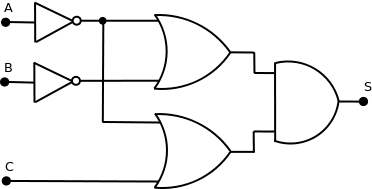
\includegraphics[scale=0.5]{CircPortas.png}}
    \caption{Diagrama l�gico correspondente � equa��o 1.}
\end{figure}

ou em dupla coluna:\\

\par\vspace{\baselineskip}
\begin{figure} [htbp!]
 \center
  \subfigure[ref1][Legenda1]{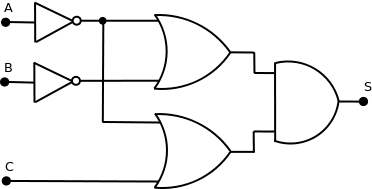
\includegraphics[width=6cm]{CircPortas.png}}
  \qquad
  \subfigure[ref2][Legenda2]{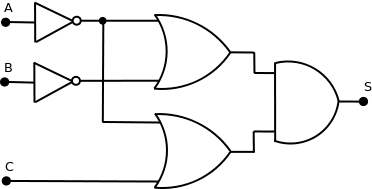
\includegraphics[width=6cm]{CircPortas.png}}
  \setlength{\captionmargin}{10pt}
  \setlength{\abovecaptionskip}{8pt}
  \captionsetup{labelsep=colon}
  \renewcommand{\figurename}{Figura}
  \caption{Imagens lado a lado}
\end{figure}

\section{Quest�es}
\par\vspace{\baselineskip}

\section{Metas}
\par\vspace{\baselineskip}

%----------------------------------------------------------------------------------------

\end{document}